\documentclass[pdflatex,sn-mathphys-num]{sn-jnl}

\usepackage{graphicx}
\usepackage{multirow}
\usepackage{amsmath,amssymb,amsfonts}
\usepackage{amsthm}
\usepackage{mathrsfs}
\usepackage[title]{appendix}
\usepackage{xcolor}
\usepackage{textcomp}
\usepackage{manyfoot}
\usepackage{booktabs}
\usepackage{algorithm}
\usepackage{algorithmicx}
\usepackage{algpseudocode}
\usepackage{listings}

\graphicspath{{figuras/}}

\raggedbottom

\begin{document}

\title[Readmisión temprana en pacientes diabéticos]{Clasificación Binaria de Readmisión Hospitalaria Temprana en Pacientes Diabéticos a partir de Registros Clínico-Administrativos: Línea de Referencia con Validación Agrupada por Paciente}

\author*[1]{\fnm{Joshua} \sur{Hincapié Llorente}}\email{hjoshua@uninorte.edu.co}

\author[1]{\fnm{Alejandro} \sur{Cantillo Escorcia}}\email{cantilloalejandro@uninorte.edu.co}

\affil*[1]{\orgdiv{Departamento de Matemáticas, Física y Ciencia de Datos}, \orgname{Universidad del Norte}, \orgaddress{\city{Barranquilla}, \country{Colombia}}}

\abstract{La readmisión hospitalaria dentro de los 30 días del alta es un indicador de calidad asistencial y una fuente de costo evitable, y su predicción a partir de registros administrativos sigue siendo un problema de desempeño modesto. Este trabajo evalúa exhaustivamente el espacio de modelado clásico sobre Diabetes 130-US Hospitals (101{,}766 encuentros de 71{,}518 pacientes), cruzando siete modelos base con cuatro estrategias de balanceo y cuatro métodos de optimización de hiperparámetros: 112 combinaciones de diseño, de las cuales 108 son ejecutables. Todas se estiman con validación cruzada anidada agrupada por paciente, de modo que ningún paciente aparece a la vez en entrenamiento y validación. La mejor configuración, XGBoost con ADASYN y Random Search, alcanza un AUC-PR de 0.2267 $\pm$ 0.0153 en el bucle externo y 0.2285 en el conjunto de prueba reservado, frente a 0.2101 $\pm$ 0.0117 de la línea base logística. El hallazgo de la línea de referencia es negativo: aunque la prueba de Friedman rechaza la igualdad global de los siete modelos ($\chi^2_F = 28.54$, $p < 0.001$), la de Nemenyi no separa a XGBoost de Random Forest ($p = 1.000$), la de DeLong entre los tres finalistas no detecta ninguna diferencia ($p \geq 0.722$) y la variabilidad por semilla del mejor modelo (0.0041 de AUC-PR) supera en un factor de 4.5 la distancia que lo separa del segundo (0.0009). Las optimizaciones computacionales reducen el tiempo de ajuste entre 2.0 y 6.7 veces sin pérdida de desempeño.}

\keywords{Readmisión hospitalaria, Clasificación desbalanceada, Validación cruzada agrupada, Comparación estadística de modelos, AUC-PR}

\maketitle

\section{Introducción}\label{sec:intro}

La readmisión hospitalaria no planificada dentro de los 30 días posteriores al alta es, desde hace más de una década, uno de los indicadores con los que los sistemas de salud miden la calidad de la atención. El trabajo de Jencks y colaboradores \cite{bib_jencks} estimó que cerca de una quinta parte de los beneficiarios de Medicare dados de alta volvía al hospital dentro de ese plazo, con un costo anual del orden de los 17 mil millones de dólares, y ese resultado motivó programas de penalización financiera que trasladaron el problema a las instituciones. En pacientes diabéticos la cuestión es especialmente relevante: la diabetes mellitus es una de las enfermedades crónicas con mayor carga sobre los servicios hospitalarios y los pacientes que ingresan con ella presentan tasas de reingreso superiores a la media.

El atractivo de un modelo predictivo en este contexto es operativo antes que científico. Si al momento del alta fuera posible ordenar a los pacientes por riesgo de reingreso, un servicio con capacidad limitada de seguimiento podría concentrar sus recursos en quienes más lo necesitan. La dificultad es que el desempeño alcanzable con registros administrativos resulta sistemáticamente modesto. La revisión sistemática de Kansagara y colaboradores \cite{bib_kansagara} examinó 26 modelos de predicción de readmisión y encontró que la mayoría obtenía un estadístico C entre 0.60 y 0.70, con poca capacidad discriminante aprovechable en la práctica clínica. El conjunto de datos que se usa aquí, publicado por Strack y colaboradores \cite{bib_strack} a partir de diez años de registros de 130 hospitales estadounidenses, se ha convertido en una referencia habitual para este problema, y los trabajos que lo emplean reportan cifras del mismo orden \cite{bib_futoma}.

Esa combinación de bajo techo y alta demanda de aplicabilidad crea un riesgo metodológico concreto, que es el que motiva este trabajo. Cuando todas las alternativas de modelado producen métricas separadas por milésimas, la diferencia entre declarar un ganador y no declararlo depende por completo del rigor del protocolo de evaluación. Dos decisiones resultan determinantes. La primera es la unidad de observación: en este conjunto de datos la fila es el encuentro hospitalario y no el paciente, de modo que un mismo individuo aporta varios registros y las observaciones no son independientes; particionar por filas en lugar de por pacientes filtra información entre entrenamiento y validación. La segunda es el control del error de tipo I: con 108 configuraciones evaluadas, el número de comparaciones por pares posibles asciende a 5{,}778, y aplicar pruebas pareadas sin corrección produciría cerca de 289 resultados significativos por puro azar.

La contribución de esta versión del trabajo es el establecimiento riguroso de la línea de referencia. Se construye un benchmark combinatorio completo del espacio de modelado clásico sobre este problema, estimado íntegramente con validación cruzada anidada agrupada por paciente, con el preprocesamiento y el remuestreo encapsulados dentro de cada pliegue, y se somete el resultado a la secuencia estadística jerárquica que corresponde a su escala: prueba ómnibus de Friedman, post-hoc de Nemenyi con diagrama de diferencia crítica, comparaciones dirigidas de DeLong con corrección por multiplicidad, intervalos bootstrap BCa remuestreados por paciente y tamaños de efecto. El modelo propuesto, que se incorporará en una versión posterior, se medirá contra esa referencia con el mismo protocolo.

Evaluamos exhaustivamente las 108 configuraciones ejecutables del espacio clásico y mostramos que, bajo un protocolo de validación que respeta la estructura de agrupamiento de los datos, ninguna de ellas puede declararse superior a las demás en el extremo superior del ranking: la ventaja aparente del mejor modelo es una fracción de su propia variabilidad por semilla aleatoria. Ese resultado fija el umbral que cualquier propuesta posterior tendrá que superar para ser creíble, y lo fija alto: no basta con quedar primero en la tabla, hay que superar el ruido.

\section{Metodología}\label{sec:metodologia}

\subsection{Descripción del problema y del conjunto de datos}\label{subsec:datos}

\textbf{Descripción general.} Se utilizó el conjunto público \emph{Diabetes 130-US Hospitals for Years 1999--2008} \cite{bib_strack}, disponible en el repositorio de aprendizaje automático de la Universidad de California en Irvine \cite{bib_uci}. Contiene 101{,}766 encuentros hospitalarios correspondientes a 71{,}518 pacientes distintos, descritos por 50 atributos: variables demográficas, administrativas, diagnósticos codificados en CIE-9, resultados de laboratorio y el estado de 23 medicamentos antidiabéticos. La unidad de observación es el encuentro, no el paciente. La variable objetivo original, \texttt{readmitted}, toma tres valores (\texttt{<30}, \texttt{>30}, \texttt{NO}) y se modela como clasificación binaria entre el reingreso antes de 30 días y el resto, que es la definición con relevancia operativa. La clase positiva representa el 11.39\% de los encuentros de entrenamiento, una razón de desbalance de 1 a 7.8.

\textbf{ETL.} \emph{Extract:} los datos se obtuvieron en formato CSV desde el repositorio UCI, junto con el archivo auxiliar \texttt{IDS\_mapping.csv} que codifica el significado de los identificadores de tipo de admisión, fuente de admisión y destino al alta; ese archivo apila tres tablas separadas por líneas en blanco y requiere lectura por bloques. El código de ausencia es el carácter \texttt{?}, que se convierte a valor nulo desactivando la interpretación por defecto de la cadena \texttt{"None"}, necesaria porque en el panel de fármacos \texttt{None} es un nivel legítimo que significa «medicamento no prescrito».

\emph{Transform:} se excluyeron 2{,}426 encuentros cuyo destino al alta es incompatible con observar un reingreso posterior, correspondientes a fallecimiento y a cuidados paliativos, lo que deja 99{,}340 registros. No se eliminaron duplicados porque no existen filas íntegramente repetidas. Las variables con ausencia masiva o varianza nula se descartaron: \texttt{weight}, con un 98.5\% de faltantes, y nueve de los 23 fármacos cuyo nivel dominante supera el umbral de variación mínima establecido, hasta dejar 40 columnas. La ausencia de \texttt{race} (2.25\%) se conservó como categoría explícita en lugar de imputarse. Los niveles categóricos poco frecuentes se agruparon para que las frecuencias esperadas sostengan las pruebas chi-cuadrado del análisis bivariado, y los diagnósticos CIE-9 se consolidaron en grupos clínicos. No se recortaron ni winsorizaron valores atípicos: el análisis univariado mostró que se concentran en las variables de utilización previa y que corresponden a pacientes con tasas de reingreso superiores a la media, es decir, a casos informativos y no a errores de captura. El escalado es robusto, con mediana e intervalo intercuartílico, y la codificación de las categóricas es \emph{one-hot}; ambos se ajustan dentro de cada pliegue de validación, nunca sobre el conjunto completo.

\emph{Load:} el conjunto final se almacenó en formato Parquet y se particionó en 79{,}473 encuentros de entrenamiento (56{,}036 pacientes) y 19{,}867 de prueba, con la restricción de que ningún paciente aparece en ambos: la partición se hizo por paciente y se verificó que la intersección es vacía. Las prevalencias resultantes son prácticamente idénticas (11.389\% y 11.391\%). La matriz que ven los modelos tiene 152 columnas, 141 procedentes de la codificación \emph{one-hot} y 11 numéricas u ordinales. La validación es cruzada anidada con cinco pliegues externos y tres internos, estratificada y agrupada por paciente. La semilla global es 42 y se propaga a \texttt{numpy}, \texttt{scikit-learn}, XGBoost, Optuna y DEAP.

\textbf{EDA exhaustivo.} El análisis descriptivo de las diez variables numéricas rechazó la normalidad en todas ellas, tanto con la prueba de Shapiro-Wilk como con la de D'Agostino-Pearson, y detectó tres variables con más del 50\% de valores en cero, hasta un máximo del 88.9\%. Esa asimetría, junto con la presencia de atípicos clínicamente plausibles, es lo que motivó el escalado robusto en lugar del estandarizado.

El análisis univariado de la variable objetivo confirmó el desbalance descrito, representado en la Figura~\ref{fig:eda_objetivo}. Pero el hallazgo más consecuente del análisis exploratorio no fue el desbalance sino la estructura de dependencia entre observaciones, resumida en la Figura~\ref{fig:eda_intra}. Los encuentros de un mismo paciente comparten casi por completo sus predictores: la varianza explicada por el paciente alcanza $\eta^2 = 0.99$ en la edad y la concordancia es de 0.9999 en el sexo, muy por encima de lo que produciría una asignación al azar de los encuentros a pacientes. La etiqueta, en cambio, no se repite con la misma fuerza. El efecto de diseño estimado por bootstrap de pacientes es de 1.395, de modo que los 79{,}473 encuentros de entrenamiento equivalen a unas 56{,}974 observaciones independientes.

El análisis bivariado midió la asociación de cada predictor con el desenlace por tres vías complementarias: un contraste de hipótesis, un tamaño de efecto y una medida de información. Quince de las 27 variables categóricas resultan significativas tras la corrección de Holm, y siete de los 28 pares examinados muestran información de interacción por encima de la suma de sus aportes individuales, lo que anticipa una ventaja pequeña para los modelos capaces de representar interacciones. La conclusión central del bivariado, sin embargo, es restrictiva: ningún predictor individual separa las clases. El mejor de ellos, el número de ingresos previos, alcanza un AUC univariado de 0.607 y aporta apenas el 2.45\% de la entropía del desenlace. Un oráculo construido sobre los perfiles discretos de los tres mejores predictores, estimado fuera de pliegue, no supera un AUC de 0.6482.

\emph{Decisiones de preprocesamiento derivadas del EDA.} Cuatro decisiones del ETL son consecuencia directa de estos hallazgos, y no elecciones por convención. Primera: la validación se agrupa por paciente, porque la Figura~\ref{fig:eda_intra} demuestra que los encuentros de un individuo no son observaciones independientes; la cuantificación del efecto aparece más abajo. Segunda: la métrica de selección es el AUC-PR y no la exactitud, porque con un 11.39\% de clase positiva un clasificador trivial que prediga siempre «no readmitido» alcanza cerca del 89\% de exactitud sin capacidad predictiva alguna \cite{bib_saito,bib_davis}. Tercera: el escalado es robusto y no se recortan atípicos, por la asimetría y el exceso de ceros descritos. Cuarta: el balanceo de clases se trata como una pregunta empírica con cuatro respuestas candidatas en lugar de aplicarse por defecto, dado que la razón de desbalance de 1 a 7.8 es moderada y no extrema.

\begin{figure}[h]
\centering
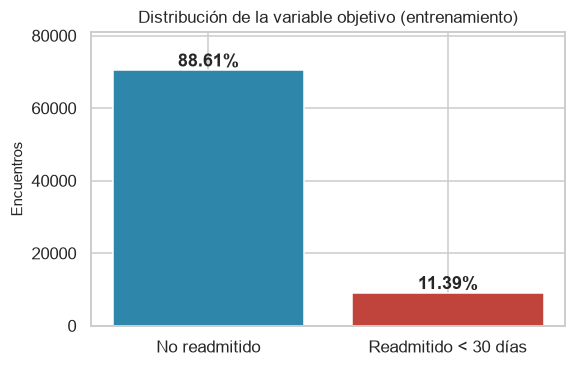
\includegraphics[width=0.72\textwidth]{fig_eda_objetivo.png}
\caption{Distribución de la variable objetivo en el conjunto de entrenamiento. La clase positiva, reingreso antes de 30 días, representa el 11.39\% de los encuentros, una razón de 1 a 7.8 que descarta la exactitud como métrica de selección.}
\label{fig:eda_objetivo}
\end{figure}

\begin{figure}[h]
\centering
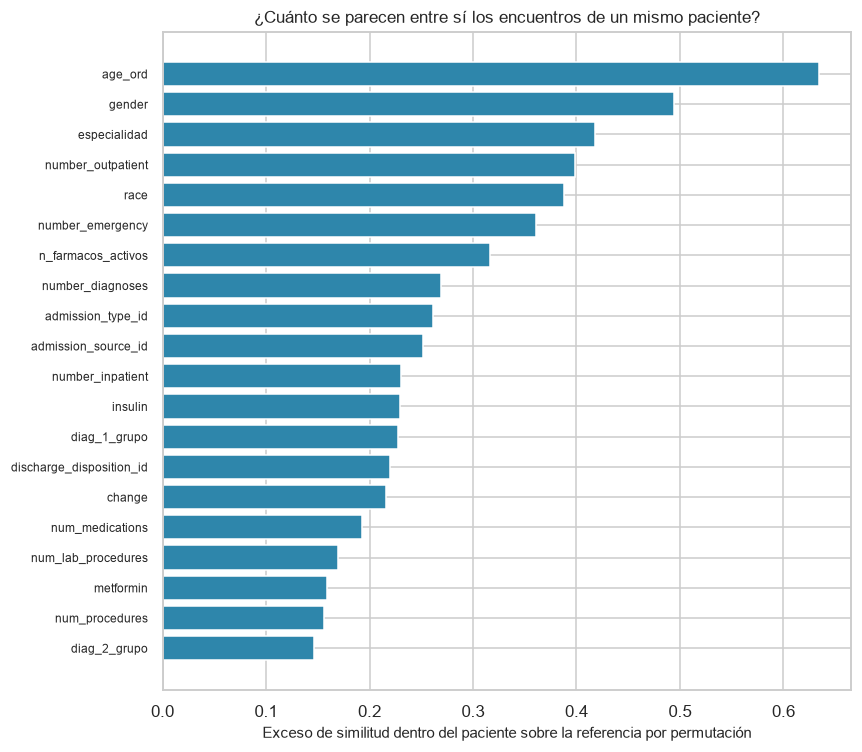
\includegraphics[width=0.95\textwidth]{fig_eda_intrapaciente.png}
\caption{Similitud entre los encuentros de un mismo paciente, contrastada contra una permutación que rompe la correspondencia encuentro-paciente. Los predictores se repiten casi íntegramente dentro del paciente mientras la etiqueta no lo hace, lo que obliga a agrupar la validación cruzada por paciente.}
\label{fig:eda_intra}
\end{figure}

\subsection{Modelos de referencia}\label{subsec:sota}

Se compararon los siete modelos de clasificación del programa del curso, cada uno cruzado con las cuatro estrategias de balanceo y los cuatro métodos de optimización descritos más abajo. La elección del conjunto no es arbitraria: cubre las tres familias de hipótesis que el análisis exploratorio identificó como relevantes para este problema, es decir, modelos lineales en el logit, modelos basados en distancias y modelos capaces de representar interacciones mediante particiones del espacio.

\textbf{Regresión logística con regularización L1 y L2} \cite{bib_tibshirani}. Es el modelo lineal generalizado canónico para un desenlace binario y cumple aquí el papel de patrón de medida: su forma funcional coincide exactamente con el supuesto que el análisis bivariado puso a prueba, de modo que su desempeño separa lo que el problema concede a una relación aditiva en el logit de lo que exige estructura adicional. Minimiza la verosimilitud negativa penalizada
\begin{equation}
\min_{\beta_0,\,\beta} \; \sum_{i=1}^{n}\Big[-y_i(\beta_0 + x_i^\top\beta) + \log\big(1+e^{\beta_0 + x_i^\top\beta}\big)\Big] + \lambda\,\Omega(\beta),
\label{eq:logistica}
\end{equation}
con $\Omega(\beta)=\lVert\beta\rVert_1$ en la variante L1 y $\Omega(\beta)=\tfrac{1}{2}\lVert\beta\rVert_2^2$ en la L2. Se exploró $C = 1/\lambda \in \{0.001, 0.01, 0.1, 1, 10, 100\}$ en escala logarítmica, cruzado con ambas penalizaciones, mediante el solucionador \texttt{liblinear} \cite{bib_liblinear}.

\textbf{Clasificador bayesiano ingenuo} \cite{bib_zhang}. Se incluye como cota inferior informativa: su supuesto de independencia condicional entre predictores es precisamente el que la matriz de interacciones del análisis bivariado contradice, de modo que su distancia respecto al resto cuantifica cuánto cuesta ignorar la dependencia entre variables. Asigna la clase que maximiza
\begin{equation}
\hat{y} = \arg\max_{c\in\{0,1\}} \; P(c)\prod_{j=1}^{p} P(x_j \mid c),
\label{eq:bayes}
\end{equation}
y se ajustó el parámetro de suavizado sobre $\{10^{-9}, 10^{-7}, \dots, 10^{-1}\}$.

\textbf{$k$ vecinos más cercanos} \cite{bib_cover}. Es el representante de los métodos basados en distancias y no asume ninguna forma funcional, lo que lo hace un contraste útil frente a los modelos paramétricos. Su regla de decisión es la mayoría ponderada entre los $k$ vecinos más próximos,
\begin{equation}
\hat{P}(y=1\mid x) = \frac{\sum_{i \in \mathcal{N}_k(x)} w_i\,\mathbb{1}[y_i = 1]}{\sum_{i \in \mathcal{N}_k(x)} w_i},
\qquad w_i = \frac{1}{d(x, x_i)},
\label{eq:knn}
\end{equation}
con $k \in \{11, 21, 51, 101\}$ y pesos uniformes o inversos a la distancia. La estrategia \texttt{class\_weight} no tiene equivalente en este modelo, porque su predicción es un voto entre vecinos sin término de pérdida que ponderar; las cuatro combinaciones afectadas se registran explícitamente como inviables.

\textbf{Árbol de decisión} \cite{bib_breiman_cart}. Primer modelo capaz de representar interacciones y de capturar relaciones no monótonas, como la que el análisis bivariado detectó en la edad. Cada división maximiza el descenso de impureza de Gini,
\begin{equation}
\Delta i(s,t) = i(t) - p_L\,i(t_L) - p_R\,i(t_R),
\qquad i(t) = 1 - \sum_{c} p(c\mid t)^2,
\label{eq:arbol}
\end{equation}
con profundidad máxima en $\{3, 5, 8, \text{sin límite}\}$ y mínimo de muestras por hoja en $\{10, 50, 200\}$.

\textbf{Random Forest} \cite{bib_breiman_rf}. Promedia árboles ajustados sobre muestras bootstrap con selección aleatoria de predictores en cada división, lo que reduce la varianza del árbol individual sin aumentar su sesgo de forma apreciable:
\begin{equation}
\hat{P}(y=1\mid x) = \frac{1}{T}\sum_{t=1}^{T} \hat{P}_t(y=1\mid x).
\label{eq:rf}
\end{equation}
Se exploraron $T \in \{100, 300\}$ árboles, profundidad en $\{5, 10, \text{sin límite}\}$ y número de predictores por división en $\{\sqrt{p}, 0.3p\}$.

\textbf{XGBoost} \cite{bib_chen}. Potenciación de gradiente con regularización explícita del tamaño del árbol, que es la referencia habitual en datos tabulares. Ajusta de forma secuencial el objetivo regularizado
\begin{equation}
\mathcal{L} = \sum_{i=1}^{n} \ell\big(y_i, \hat{y}_i^{(t-1)} + f_t(x_i)\big) + \gamma T_t + \tfrac{1}{2}\lambda\lVert w_t\rVert^2,
\label{eq:xgb}
\end{equation}
donde $T_t$ es el número de hojas del árbol $t$ y $w_t$ sus pesos. Se exploraron tasa de aprendizaje en $\{0.03, 0.1, 0.3\}$, profundidad en $\{3, 6\}$ y número de estimadores en $\{200, 600\}$, con el método de histogramas y parada temprana. Como no acepta \texttt{class\_weight}, se usa su equivalente directo \texttt{scale\_pos\_weight} fijado en la razón de desbalance.

\textbf{Máquinas de vectores de soporte} \cite{bib_cortes}. Completan el conjunto con un criterio de margen máximo. Resuelven el problema primal con margen suave
\begin{equation}
\min_{w,b,\xi} \; \tfrac{1}{2}\lVert w\rVert^2 + C\sum_{i=1}^{n}\xi_i
\quad \text{sujeto a} \quad y_i\big(w^\top\phi(x_i)+b\big) \geq 1-\xi_i, \;\; \xi_i \geq 0.
\label{eq:svm}
\end{equation}
Dado el tamaño de muestra, que haría prohibitivo el costo cuadrático del núcleo completo, se empleó la formulación lineal \texttt{LinearSVC} con $C \in \{0.01, 0.1, 1, 10\}$, y las probabilidades se obtuvieron por escalado de Platt \cite{bib_platt}.

\textbf{Estrategias de balanceo.} Se compararon cuatro: ausencia de tratamiento como línea base; SMOTE \cite{bib_smote}, que genera instancias sintéticas interpolando entre vecinos de la clase minoritaria; ADASYN \cite{bib_adasyn}, que concentra la generación en las instancias más difíciles de aprender según una distribución de densidad; y la reponderación \texttt{class\_weight="balanced"}, que penaliza los errores en proporción inversa a la frecuencia de cada clase. Las dos primeras se aplican exclusivamente dentro del pliegue de entrenamiento, mediante la tubería de \texttt{imbalanced-learn} \cite{bib_imblearn}, porque interpolan entre vecinos y aplicarlas antes de particionar filtraría información del pliegue de validación.

\textbf{Métodos de optimización de hiperparámetros.} Grid Search exhaustivo sobre la rejilla declarada; Random Search \cite{bib_bergstra_random}, cuyo argumento teórico es que si pocos hiperparámetros dominan el desempeño el muestreo aleatorio explora más valores distintos de esos pocos con el mismo presupuesto; optimización bayesiana con Optuna \cite{bib_optuna}, cuyo modelo sustituto es un estimador de Parzen estructurado en árbol \cite{bib_bergstra_tpe} que estima por separado la densidad de las configuraciones buenas y malas y cuya función de adquisición es la mejora esperada, privilegiando la explotación de regiones ya prometedoras; y un algoritmo genético con DEAP \cite{bib_deap}, con selección por torneo de tamaño 3, cruce uniforme y mutación gaussiana, elitismo mediante salón de la fama y seguimiento de la diversidad genética por generación como indicador de convergencia prematura. Se añadió eliminación sucesiva \cite{bib_jamieson,bib_hyperband} dentro de la optimización bayesiana, con el número de pliegues internos evaluados como medida de fidelidad.

\subsection{Modelo propuesto}\label{subsec:propuesto}

\textcolor{blue!55!black}{\textbf{Pendiente de desarrollo.}} \emph{El modelo propuesto y su comparación frente a los modelos de referencia se incorporarán en una versión posterior de este manuscrito. Lo que esta subsección documenta hasta ahora es el protocolo de evaluación sobre el que esa comparación se hará, que ya está fijado y validado, de modo que el modelo propuesto se medirá con el mismo rasero que los 108 de referencia y sus cifras serán directamente comparables con las de la Sección~\ref{sec:resultados}.}

Fijar el protocolo antes que el modelo no es un orden accidental. En un problema donde todas las alternativas quedan separadas por milésimas, el resultado depende más de cómo se valida que de qué se valida, y un protocolo decidido después de ver los resultados no sería creíble. Los tres elementos siguientes son los que lo componen.

\emph{Primero, la validación agrupada por paciente en ambos niveles del anidamiento.} Tanto el bucle externo como el interno usan \texttt{StratifiedGroupKFold} sobre el identificador de paciente, y el submuestreo que abarata la búsqueda se hace también por paciente y no por fila. El efecto de omitir esta precaución se midió de forma directa: particionar por filas en lugar de por pacientes infla el AUC-PR en 0.0127 en Random Forest y en 0.0030 en $k$-NN, y el AUC-ROC en 0.0057 y 0.0017 respectivamente. Ese sesgo es del mismo orden que las diferencias entre modelos que el experimento pretende detectar, lo que convierte el agrupamiento en una condición necesaria para que la comparación signifique algo.

\emph{Segundo, el encapsulamiento completo del preprocesamiento y del remuestreo dentro del pliegue.} La imputación, el escalado robusto, la codificación \emph{one-hot} y el sobremuestreo sintético se ajustan únicamente con los datos de entrenamiento de cada pliegue. La métrica que se reporta proviene siempre del bucle externo, nunca del valor óptimo hallado en el interno, que está contaminado por la propia selección de hiperparámetros \cite{bib_cawley,bib_varma}.

\emph{Tercero, el esquema de fidelidad reducida y su verificación.} Para que el experimento quepa en un presupuesto razonable, la búsqueda interna de los modelos económicos se realiza sobre una submuestra del 25\% de los pacientes. El supuesto que introduce ese atajo es que el orden relativo entre configuraciones se conserva al reducir la muestra, y el supuesto no se da por bueno: se repite la búsqueda con fidelidad completa y se emparejan las corridas que solo difieren en ese factor. En los modelos económicos, las 16 corridas emparejadas difieren como máximo 0.0070 de AUC-PR, con una media de 0.0012, y las 16 quedan dentro del ruido entre pliegues; en los costosos, las 12 emparejadas difieren como máximo 0.0049. El atajo, por tanto, no altera las conclusiones.

El Algoritmo~\ref{alg:protocolo} resume el procedimiento.

\begin{algorithm}
\caption{Evaluación anidada agrupada por paciente de una configuración}\label{alg:protocolo}
\begin{algorithmic}[1]
\Require Encuentros $X$, etiquetas $y$, identificadores de paciente $g$, configuración $(m, b, o)$ de modelo, balanceo y optimizador, presupuesto $B$
\Ensure Métricas fuera de muestra $\mu \pm \sigma$ y costo computacional
\State $\mathcal{F} \gets \textsc{StratifiedGroupKFold}(X, y, g, K_{\text{ext}}=5)$
\For{cada pliegue externo $(\mathcal{T}_k, \mathcal{V}_k) \in \mathcal{F}$}
    \State $\mathcal{S}_k \gets$ submuestra de $\mathcal{T}_k$ por paciente según la fidelidad de $m$
    \State $\mathcal{F}' \gets \textsc{StratifiedGroupKFold}(\mathcal{S}_k, K_{\text{int}}=3)$
    \State $\theta_k^\star \gets \arg\max_{\theta \in o(B)} \; \textsc{AUC-PR}\big(\textsc{Tubería}(m,b,\theta), \mathcal{F}'\big)$
    \Comment{bucle interno: solo elige $\theta$}
    \State Ajustar $\textsc{Tubería}(m, b, \theta_k^\star)$ sobre $\mathcal{T}_k$ completo
    \Comment{preprocesamiento y balanceo dentro del pliegue}
    \State $\mu_k \gets$ métricas sobre $\mathcal{V}_k$
    \Comment{bucle externo: única fuente de la métrica reportada}
\EndFor
\State \Return $\big(\overline{\mu},\; \mathrm{sd}(\mu),\; \{\theta_k^\star\},\; \text{tiempos}\big)$
\end{algorithmic}
\end{algorithm}

\subsection{Configuración experimental}\label{subsec:config}

\textbf{Métricas.} La métrica de selección es el AUC-PR, es decir la precisión media. La razón es el desbalance: el AUC-ROC normaliza los falsos positivos por una clase mayoritaria que aquí es ocho veces más grande, lo que comprime las diferencias en la región de interés, mientras que la curva de precisión-exhaustividad parte de una línea horizontal en la prevalencia y refleja directamente el costo de revisar pacientes que no van a reingresar \cite{bib_saito,bib_davis}. Se reportan además el AUC-ROC, por comparabilidad con la literatura de readmisión, la exactitud balanceada, y el coeficiente de Brier \cite{bib_brier} junto con el error de calibración esperado para evaluar la calidad de las probabilidades. La exactitud se reporta solo como referencia, porque un clasificador trivial alcanza el 89\%.

\textbf{Hardware y software.} Todos los experimentos se ejecutaron en un único equipo con cuatro núcleos físicos (ocho lógicos) y tarjeta gráfica AMD. La ausencia de CUDA impide medir el factor de aceleración por GPU de XGBoost, de modo que la totalidad del experimento corre en CPU y así se declara. La paralelización se organiza en dos niveles sin sobresuscripción, con \texttt{n\_jobs = 4} y reparto entre pliegues para los modelos que no paralelizan internamente; la aceleración medida es de 1.9 veces con cuatro núcleos físicos, un 48\% de eficiencia respecto al máximo teórico. Las versiones exactas de las 172 dependencias están fijadas en \texttt{requirements.txt}; las principales son \texttt{scikit-learn} 1.9.1 \cite{bib_sklearn}, \texttt{xgboost} 3.4.1, \texttt{imbalanced-learn} 0.14.2, \texttt{optuna} 5.0.0, \texttt{deap} 1.4.4, \texttt{shap} 0.52.0, \texttt{lime} 0.2.0.1, \texttt{numpy} 2.5.3, \texttt{pandas} 3.0.5, \texttt{scipy} 1.18.1 y \texttt{scikit-posthocs} 0.17.0.

\textbf{Medición del tiempo.} Se registran por separado, en segundos de reloj de pared, el tiempo de búsqueda de hiperparámetros, el de ajuste final del modelo sobre el pliegue completo y el de inferencia sobre el pliegue de validación, además del tiempo real y el tiempo de trabajo acumulado. Cada una de las 108 corridas queda registrada en una tabla maestra con sus hiperparámetros finales, sus métricas por pliegue, sus tiempos, su semilla y sus condiciones de paralelización. El experimento completo consumió 22.9 horas de cómputo.

\textbf{Repeticiones.} La variabilidad entre pliegues se reporta como desviación estándar sobre los cinco pliegues externos. La sensibilidad a la semilla aleatoria se evaluó repitiendo la mejor configuración con las semillas 42, 7 y 2026. Esta medición resulta decisiva para la interpretación de los resultados y se retoma en la Sección~\ref{sec:resultados}.

\section{Resultados}\label{sec:resultados}

\subsection{Desempeño y costo}

La Tabla~\ref{tab:resultados} resume la mejor configuración de cada uno de los siete modelos, con las métricas procedentes del bucle externo. El orden reproduce con fidelidad la jerarquía que el análisis exploratorio anticipaba: los dos modelos capaces de representar interacciones ocupan los primeros puestos, los lineales y el de márgenes quedan en la zona media y el clasificador bayesiano ingenuo cierra la tabla, a una distancia que cuantifica el costo de suponer independencia condicional entre predictores. La Figura~\ref{fig:ranking} muestra la misma comparación con sus barras de error.

Lo relevante no es ese orden, sino su escala. Los siete modelos se reparten en un intervalo de 0.027 de AUC-PR, y los dos primeros están separados por 0.0009, menos de una milésima. Para contextualizar esa distancia: la desviación estándar entre pliegues del mejor modelo es de 0.0153, su error estándar de la media es de 0.0068, y al repetir esa misma configuración con tres semillas distintas el AUC-PR recorre un rango de 0.0041. La diferencia entre el primer y el segundo modelo es, por tanto, aproximadamente 4.5 veces menor que la variabilidad que produce cambiar la semilla aleatoria del mismo modelo. Ninguna conclusión sobre el ordenamiento del extremo superior sobrevive a esa comparación.

En la dimensión de costo la separación sí es sustancial, como muestra la Figura~\ref{fig:costo}. Los modelos económicos ajustan en torno a los 26--28 segundos frente a los 241--242 de los dos ensambles, y la diferencia en inferencia es más marcada todavía: $k$-NN requiere 50.8 segundos porque su costo está íntegramente en la consulta, mientras el resto se mantiene entre 1.4 y 3.1 segundos. La lectura conjunta de ambas dimensiones es que los dos ensambles compran una ventaja de 0.016 de AUC-PR sobre la logística a cambio de multiplicar por nueve el tiempo de ajuste, y que esa ventaja, como se acaba de establecer, no es estadísticamente distinguible.

El balanceo de clases merece una mención aparte, porque su resultado es contrario a la expectativa con la que suele aplicarse. De los siete modelos, **solo XGBoost mejora al balancear**, y lo hace por 0.0024 de AUC-PR con ADASYN; los otros seis obtienen su mejor resultado sin tratamiento alguno, y algunos pierden de forma apreciable: $k$-NN cae 0.0118, el SVM 0.0072 y Random Forest 0.0049. Con una razón de desbalance de 1 a 7.8, que es moderada, el sobremuestreo sintético introduce más distorsión que señal. Y la única ganancia del experimento merece una advertencia adicional: esos 0.0024 coinciden en magnitud con la cota del sesgo de parada temprana descrito en la Sección~\ref{sec:conclusiones}, que afecta precisamente a las corridas de XGBoost con remuestreo, de modo que no puede descartarse que sean un artefacto de ese sesgo en lugar de un efecto del balanceo.

\begin{table}[h]
\caption{Mejor configuración de cada modelo base, con métricas del bucle externo de la validación anidada agrupada por paciente (media $\pm$ desviación estándar sobre cinco pliegues) y tiempos en segundos. La fila de la línea base corresponde al modelo de referencia del capítulo 7, con penalización L1, $C = 0.1$ y reponderación por clase.}\label{tab:resultados}
\begin{tabular}{@{}llccccc@{}}
\toprule
Modelo & Balanceo / Optim. & AUC-PR & AUC-ROC & Búsq. & Ajuste & Infer. \\
\midrule
XGBoost        & ADASYN / Random   & \textbf{0.2267} $\pm$ 0.0153 & 0.6689 $\pm$ 0.0066 & 476.3 & 242.0 & 2.51 \\
Random Forest  & Ninguno / DEAP    & 0.2258 $\pm$ 0.0170 & \textbf{0.6703} $\pm$ 0.0087 & 668.6 & 240.8 & 3.09 \\
SVM lineal     & Ninguno / Grid    & 0.2145 $\pm$ 0.0133 & 0.6626 $\pm$ 0.0080 & 332.7 & \textbf{28.0} & 1.41 \\
Logística      & Ninguno / Optuna  & 0.2110 $\pm$ 0.0131 & 0.6619 $\pm$ 0.0079 & 944.6 & 68.0 & 2.38 \\
$k$-NN         & Ninguno / Grid    & 0.2058 $\pm$ 0.0160 & 0.6504 $\pm$ 0.0105 & 205.1 & 26.5 & 50.84 \\
Árbol          & Ninguno / Grid    & 0.2034 $\pm$ 0.0106 & 0.6522 $\pm$ 0.0064 & 264.0 & 28.1 & 1.44 \\
Naive Bayes    & Ninguno / Random  & 0.1995 $\pm$ 0.0115 & 0.6479 $\pm$ 0.0100 & 266.6 & \textbf{25.5} & 1.74 \\
\midrule
\emph{Línea base} & \emph{class\_weight / Grid} & \emph{0.2101} $\pm$ 0.0117 & \emph{0.6634} $\pm$ 0.0065 & --- & \emph{15.2} & --- \\
\botrule
\end{tabular}
\end{table}

\begin{figure}[h]
\centering
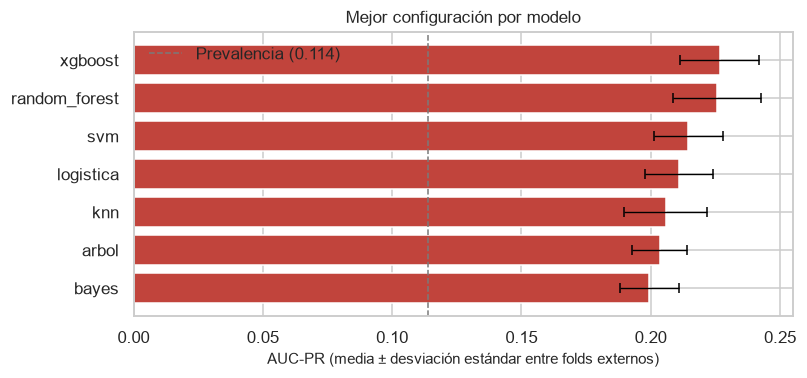
\includegraphics[width=0.85\textwidth]{fig_ranking_modelos.png}
\caption{Mejor configuración por modelo con su desviación estándar entre pliegues externos. El solapamiento de las barras de error en los primeros puestos anticipa el resultado de las pruebas formales: el experimento no tiene resolución para ordenar el extremo superior.}
\label{fig:ranking}
\end{figure}

\begin{figure}[h]
\centering
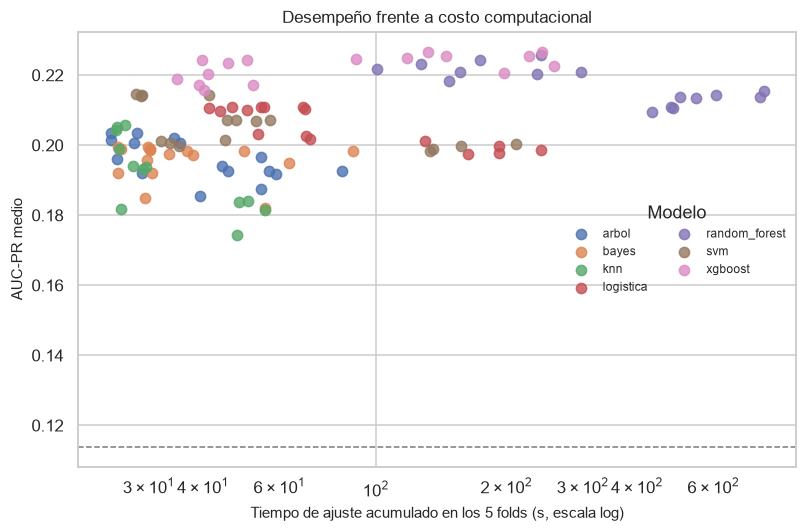
\includegraphics[width=0.85\textwidth]{fig_desempeno_costo.png}
\caption{Desempeño frente a costo computacional de las configuraciones evaluadas. Los ensambles compran una ventaja de desempeño inferior a la variabilidad por semilla a cambio de un orden de magnitud en tiempo de ajuste.}
\label{fig:costo}
\end{figure}

\subsection{Comparación de los métodos de optimización}

Promediando sobre todos los modelos y balanceos, los cuatro optimizadores quedan prácticamente empatados en calidad: Optuna alcanza un AUC-PR medio de 0.2062, Random Search 0.2061, Grid Search 0.2057 y el algoritmo genético 0.2031, con un presupuesto medio idéntico de 10.4 evaluaciones. El rango completo es de 0.0031, de nuevo inferior al ruido por semilla. En eficiencia por unidad de presupuesto, en cambio, el orden se invierte y la diferencia sí es apreciable: Grid Search rinde 0.0217 de AUC-PR por minuto de búsqueda frente a 0.0140 de Optuna, que resulta el más lento porque es intrínsecamente secuencial y, con la poda activa, tampoco paraleliza sus pliegues internos. La Figura~\ref{fig:optim} presenta la comparación y la Figura~\ref{fig:conv} las curvas de convergencia en cualquier momento.

La conclusión es específica de este problema y conviene no generalizarla: la superficie de validación de estos modelos es una meseta, con variaciones de milésimas en toda la región razonable del espacio de hiperparámetros, y sobre una meseta la búsqueda informada no tiene nada que explotar. El argumento teórico que favorece a los métodos bayesianos y evolutivos presupone una superficie con estructura aprovechable; aquí esa premisa no se cumple.

\begin{figure}[h]
\centering
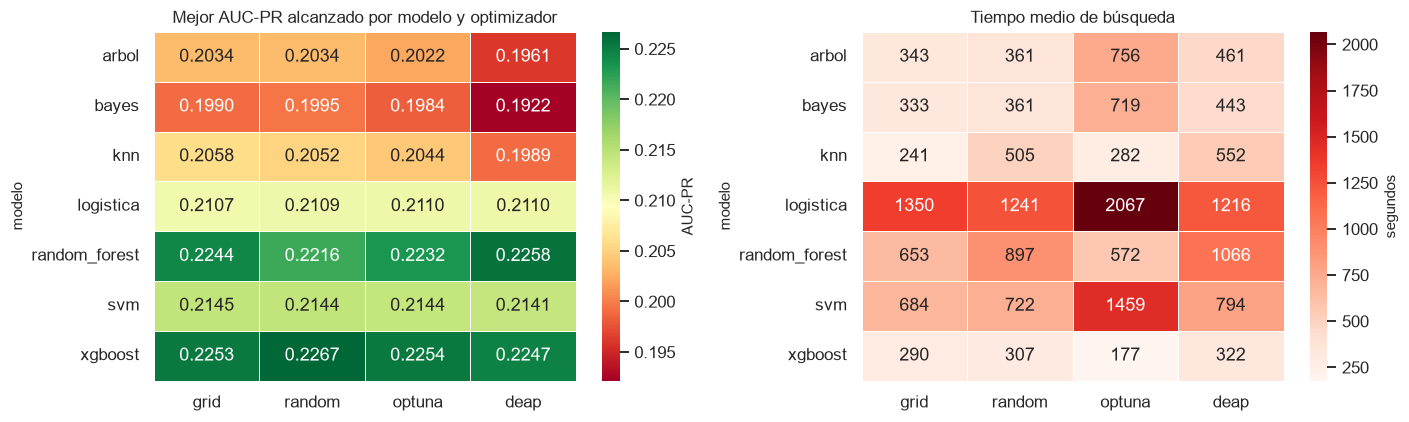
\includegraphics[width=0.95\textwidth]{fig_optimizadores.png}
\caption{Mejor AUC-PR alcanzado y tiempo medio de búsqueda por modelo y optimizador. Las diferencias de calidad entre métodos son inferiores al ruido por semilla; las de costo no.}
\label{fig:optim}
\end{figure}

\begin{figure}[h]
\centering
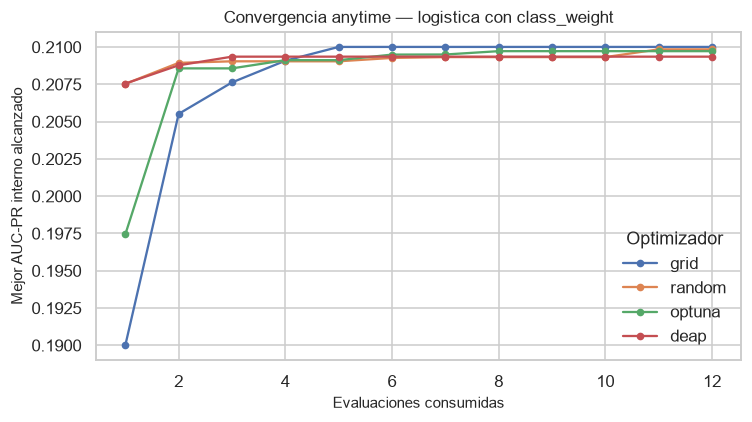
\includegraphics[width=0.78\textwidth]{fig_convergencia.png}
\caption{Convergencia en cualquier momento: mejor valor de la métrica objetivo encontrado hasta la evaluación $t$. Las trayectorias se separan poco porque la superficie de validación es una meseta.}
\label{fig:conv}
\end{figure}

\subsection{Optimización computacional}

Las sustituciones de implementación aplicadas a cada familia producen reducciones de tiempo sin pérdida de desempeño, verificadas con la métrica en la misma tabla. En la logística, el cambio del solucionador SAGA \cite{bib_saga} a \texttt{liblinear} reduce el ajuste de 55.6 a 8.3 segundos, un factor de 6.7, con un AUC-PR idéntico de 0.23. El paso de matriz dispersa a densa acelera el árbol 2.4 veces y Random Forest 3.6, sin alterar la métrica. En $k$-NN el ajuste no cambia, porque el modelo solo almacena los datos, pero la inferencia pasa de 50.3 a 8.0 segundos, un factor de 6.3, que es donde ese modelo gasta su tiempo. En XGBoost, el método de histogramas reduce el ajuste de 13.6 a 7.1 segundos y la parada temprana lo lleva a 6.7, con el AUC-PR subiendo de 0.2367 a 0.2462. El consumo máximo de memoria se mantiene entre 182 y 201 MB en todas las variantes, de modo que ninguna de estas aceleraciones se paga con memoria.

\subsection{Comparación estadística}

La prueba ómnibus de Friedman \cite{bib_friedman} sobre los rangos de los siete modelos en los cinco pliegues externos rechaza la hipótesis de equivalencia global, con $\chi^2_F = 28.54$ sobre 6 grados de libertad y $p = 7.4\times10^{-5}$. Ese rechazo autoriza el análisis post-hoc, pero no dice qué modelos difieren.

La prueba de Nemenyi \cite{bib_nemenyi,bib_demsar} lo responde, y su respuesta es la pieza central de este trabajo. Con solo cinco bloques la diferencia crítica es de 4.028 posiciones de rango, sobre rangos medios que van de 1.6 a 7.0. El diagrama de diferencia crítica de la Figura~\ref{fig:cd} no agrupa a los siete modelos en un único conjunto indistinguible, pero tampoco separa a los que importan: XGBoost y Random Forest comparten el primer puesto con rango medio idéntico y quedan unidos por la barra ($p = 1.000$), y la separación que la prueba detecta ocurre en el extremo opuesto, entre esos dos y el clasificador bayesiano ($p = 0.0015$) o el árbol ($p = 0.0345$). El experimento tiene poder para distinguir un buen modelo de uno malo, no para ordenar el extremo superior, que es precisamente donde se tomaría la decisión.

Una advertencia sobre la validez de estas dos pruebas. El representante de cada modelo se eligió tomando el máximo de AUC-PR entre sus dieciséis configuraciones, y esos mismos valores por pliegue sirvieron después de bloques: es inferencia posterior a una selección, de modo que ambos estadísticos son anticonservadores. La dispersión interna de cada modelo entre sus propias configuraciones, entre 0.011 y 0.032 de AUC-PR, es mayor que las diferencias que las pruebas declaran.

Ese sesgo, sin embargo, no es el que sostiene la conclusión, y puede comprobarse con los mismos datos. Repitiendo el contraste con dos reglas que no miran el desempeño antes de elegir el representante —una configuración preespecificada idéntica para los siete modelos, y el promedio de las dieciséis configuraciones de cada modelo pliegue a pliegue— el resultado se mantiene: los estadísticos de Friedman quedan en 28.11 y 28.46 frente a 28.54 del contraste principal, con $p$ de $8.9\times10^{-5}$ y $7.7\times10^{-5}$, y en ninguna de las tres reglas la diferencia crítica llega a separar al primero del segundo. Con las dos primeras reglas XGBoost y Random Forest empatan en rango medio; con la tercera quedan a una posición de distancia, cuando la diferencia crítica es de cuatro. El extremo superior resulta indistinguible con cualquiera de las tres.

Las comparaciones dirigidas se reservaron para los tres finalistas evaluados sobre el conjunto de prueba, mediante la prueba de DeLong \cite{bib_delong}, apropiada aquí porque las tres curvas ROC se calculan sobre las mismas observaciones y sus errores están correlacionados. Ninguna de las tres comparaciones resulta significativa: las diferencias de AUC son de 0.00015, 0.00084 y 0.00099, con $p$ crudos de 0.941, 0.754 y 0.722, que tras la corrección de Holm \cite{bib_holm} y el control de la tasa de falsos descubrimientos \cite{bib_bh} quedan en 1.000 y 0.941. Los intervalos de confianza BCa \cite{bib_efron} al 95\%, construidos con mil réplicas remuestreando pacientes completos y no filas, se solapan ampliamente: el AUC-PR de XGBoost con ADASYN cae en $[0.2114,\, 0.2499]$ y el de Random Forest en $[0.2115,\, 0.2489]$, como muestra la Figura~\ref{fig:bca}.

Los tamaños de efecto completan el cuadro y resuelven una aparente tensión. La delta de Cliff \cite{bib_cliff}, consistente con el uso de rangos, asigna magnitud grande a las comparaciones contra los modelos del fondo de la tabla ($-0.92$ frente al clasificador bayesiano, $-0.84$ frente al árbol, $-0.68$ frente a la logística) y magnitud insignificante a la que separa a XGBoost de Random Forest ($-0.12$). Conviene leer esas etiquetas con cuidado: una delta de $-0.92$ indica dominancia estocástica casi completa entre pliegues, pero la diferencia absoluta correspondiente es de 0.027 de AUC-PR. La dominancia en el ordenamiento y la relevancia práctica son dimensiones distintas, y con cinco observaciones por grupo la delta solo puede tomar múltiplos de 0.08, lo que la hace un instrumento grueso.

\begin{figure}[h]
\centering
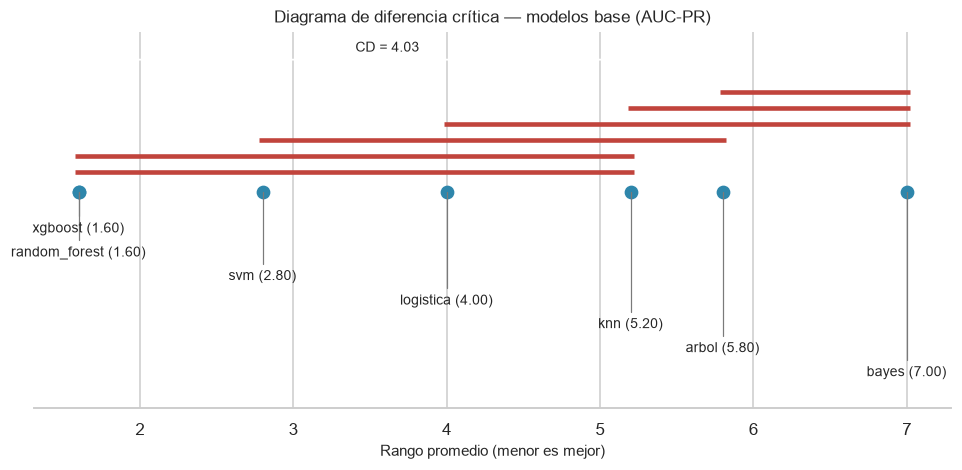
\includegraphics[width=0.80\textwidth]{fig_cd_nemenyi.png}
\caption{Diagrama de diferencia crítica de la prueba de Nemenyi sobre los siete modelos y los cinco pliegues externos. Con $\mathrm{CD} = 4.028$, XGBoost y Random Forest quedan unidos en el primer puesto; la prueba solo separa a esos dos del clasificador bayesiano y del árbol.}
\label{fig:cd}
\end{figure}

\begin{figure}[h]
\centering
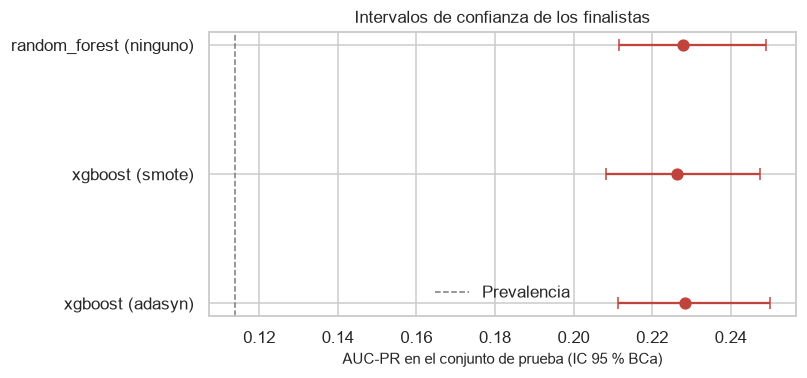
\includegraphics[width=0.80\textwidth]{fig_intervalos_bca.png}
\caption{Intervalos de confianza BCa al 95\% de los tres finalistas sobre el conjunto de prueba, con mil réplicas bootstrap remuestreadas por paciente. El solapamiento es prácticamente total.}
\label{fig:bca}
\end{figure}

\subsection{Modelo final sobre el conjunto de prueba}

La configuración de mejor AUC-PR en el bucle externo se ajustó con todo el entrenamiento y se evaluó una única vez sobre los 19{,}867 encuentros reservados. Obtiene un AUC-ROC de 0.6650 y un AUC-PR de 0.2285, cifras coherentes con las del bucle externo y con el techo de 0.6482 que el oráculo por perfiles había estimado, lo que indica que el modelo agota la información disponible en estos predictores. Las curvas aparecen en la Figura~\ref{fig:curvas}.

La calibración resultó mejor de lo que el protocolo anticipaba y el resultado se reporta tal como salió. El modelo sin recalibrar llega al conjunto de prueba con un error de calibración esperado de 0.0013 y una probabilidad media predicha de 0.1149 frente a una prevalencia observada de 0.1139, es decir bien calibrado. En consecuencia no había margen que recuperar: el escalado de Platt \emph{empeora} el error de calibración hasta 0.0137, un orden de magnitud, al imponer una sigmoide de dos parámetros a unas probabilidades que no la necesitaban, y la regresión isotónica \cite{bib_zadrozny} lo deja en 0.0015. El coeficiente de Brier permanece en 0.0962 en los tres casos y el AUC-PR no cambia de forma apreciable, lo que confirma que ambas transformaciones son monótonas y que el procedimiento está correctamente implementado \cite{bib_niculescu}. El modelo final se reporta, por tanto, sin recalibrar, y la recalibración queda documentada como una comprobación que resultó innecesaria.

El umbral de decisión se fija por capacidad de seguimiento y no maximizando una métrica, porque es un parámetro organizativo. Marcando al 15\% de mayor riesgo, el modelo detecta 710 de las 2{,}263 readmisiones del conjunto de prueba, con una exhaustividad del 31.4\% y una precisión del 23.8\%, es decir aproximadamente un acierto por cada cuatro pacientes señalados, frente al 11.4\% que daría la selección al azar. Al 30\% de capacidad la exhaustividad sube al 50.8\% y la precisión baja al 19.3\%. Esa tabla es la que traduce las centésimas de AUC en pacientes, y es también la que delimita con honestidad lo que este modelo puede ofrecer.

Ese umbral se calcula como un percentil de las puntuaciones del conjunto de prueba, lo que no usa sus etiquetas pero conviene verificar igualmente. Derivando el mismo percentil de las predicciones fuera de pliegue del entrenamiento, obtenidas con validación cruzada agrupada por paciente, el umbral se mueve 0.0017 (de 0.1705 a 0.1689) y la exhaustividad resultante pasa de 31.4\% a 31.8\%. El punto de operación, por tanto, no depende de haber visto el conjunto sobre el que se reporta.

El análisis de interpretabilidad con valores de Shapley \cite{bib_lundberg}, en la Figura~\ref{fig:shap}, sitúa en los primeros puestos el destino al alta y el número de ingresos previos, en coincidencia con el ranking de predictores del análisis bivariado. La comparación con LIME \cite{bib_ribeiro} exigió un ajuste metodológico que vale la pena documentar, porque condiciona cómo debe leerse. Construida sobre la matriz codificada de 152 columnas, de las que 142 son indicadoras dispersas, la explicación local resulta vacía: al perturbar, casi todas las indicadoras caen en cero, las predicciones del vecindario quedan prácticamente constantes, el modelo lineal local se aplana y los pesos obtenidos son del orden de $10^{-7}$. Declarar esas columnas como categóricas no lo resuelve, porque el problema es la dimensión y la dispersión, no el discretizador. Reconstruida sobre el espacio original de 38 predictores, con las categóricas codificadas como enteros y declaradas como tales y una función de predicción que atraviesa el pipeline completo, cada perturbación produce una combinación válida de categorías en lugar de un vector disperso imposible, y los pesos recuperan una magnitud normal, con un máximo de 0.243.

Sobre esa representación LIME sitúa en los primeros puestos el número de ingresos previos, las visitas previas a urgencias y el traslado a otra institución de hospitalización, que son las mismas variables que encabezan el ranking global del análisis bivariado. SHAP, para el mismo paciente, ordena primero el indicador de sexo y los grupos diagnósticos. La divergencia no debe leerse como un desacuerdo entre métodos sin antes descontar una asimetría del montaje: SHAP opera sobre la matriz codificada y LIME sobre el espacio original, de modo que una variable con muchos niveles reparte su contribución entre varias indicadoras en el primero y se agrega en una sola condición en el segundo. Lo que resta de la diferencia responde a que las dos técnicas contestan preguntas distintas, la desviación respecto a la predicción media frente a la pendiente local de la frontera de decisión.

Por último, el análisis de equidad del modelo de referencia muestra disparidades que merecen atención antes de cualquier uso. Con una cobertura global del 22.4\% al priorizar el 10\% de las altas, los grupos de edad extremos quedan muy desigualmente atendidos: la cobertura es del 42.0\% en el grupo de 20 a 30 años y del 6.1\% en el de 10 a 20, y los encuentros sin información de raza reciben una cobertura relativa de 0.36. Un despliegue real exigiría corregir esas brechas antes que mejorar el AUC.

\begin{figure}[h]
\centering
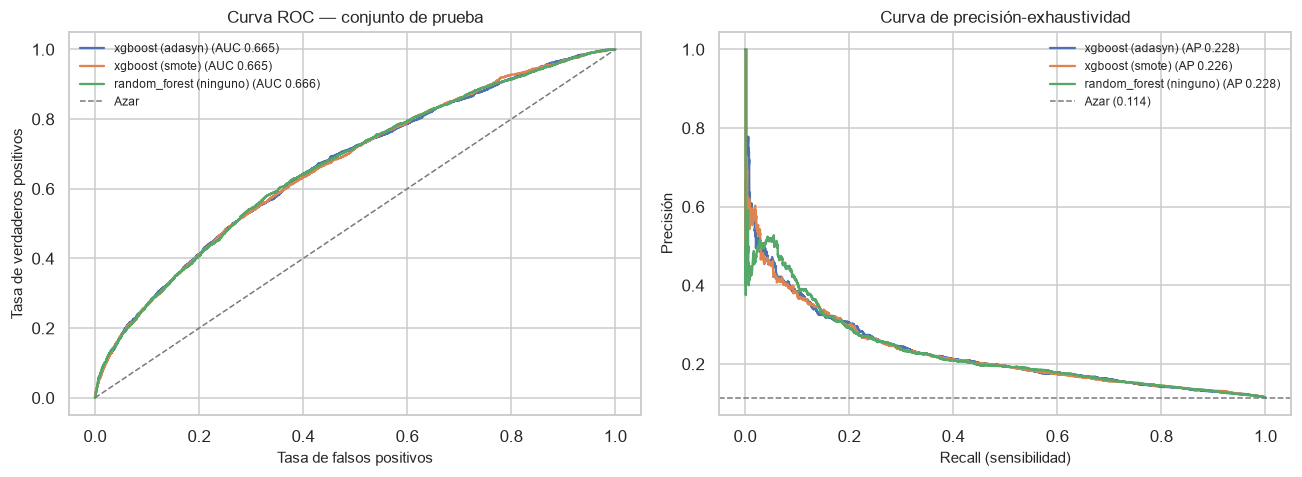
\includegraphics[width=0.95\textwidth]{fig_curvas_prueba.png}
\caption{Curva ROC y curva de precisión-exhaustividad del modelo final sobre el conjunto de prueba. La línea horizontal de la curva PR marca la prevalencia, que es el valor que alcanzaría un clasificador aleatorio.}
\label{fig:curvas}
\end{figure}

\begin{figure}[h]
\centering
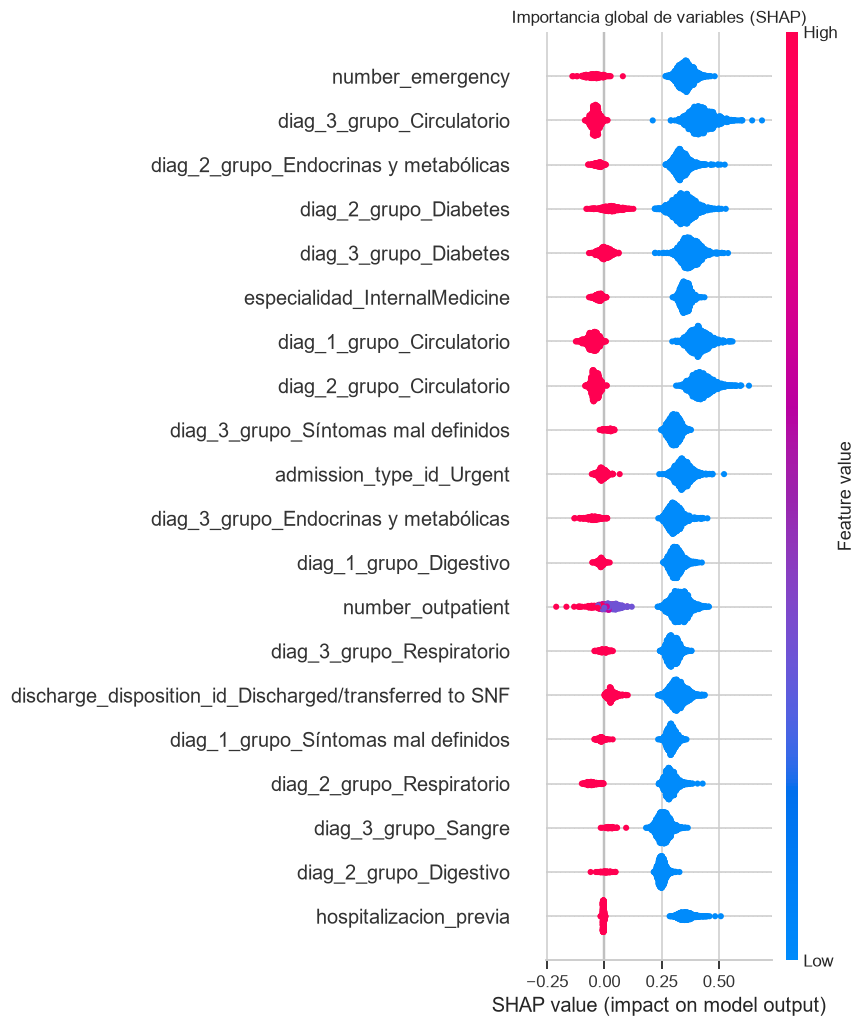
\includegraphics[width=0.85\textwidth]{fig_shap_global.png}
\caption{Importancia global de variables por valores de Shapley sobre el conjunto de prueba. El destino al alta y la utilización previa dominan la atribución, en coincidencia con el análisis bivariado.}
\label{fig:shap}
\end{figure}

\section{Conclusiones}\label{sec:conclusiones}

Esta versión del trabajo no evalúa todavía un modelo propuesto, que queda para una entrega posterior; lo que sí deja establecido es la referencia contra la que se medirá, y el resultado de establecerla conviene decirlo sin rodeos: entre los 108 modelos evaluados ninguno puede declararse mejor que los demás en el extremo superior del ranking. La prueba de Friedman rechaza la equivalencia global de los siete modelos, pero el post-hoc de Nemenyi no separa a XGBoost de Random Forest, la prueba de DeLong entre los tres finalistas no detecta diferencia alguna sobre el conjunto de prueba, los intervalos BCa se solapan casi por completo y la delta de Cliff califica de insignificante la distancia entre los dos primeros. El argumento decisivo es más simple que cualquiera de esas pruebas: la diferencia entre el primer y el segundo modelo es 4.5 veces menor que el rango que recorre el primero al cambiarle la semilla aleatoria. En la dimensión de costo computacional sí hay resultados positivos y verificables, aunque pertenecen a la ingeniería del pipeline y no a los modelos: las sustituciones de implementación aceleran el ajuste entre 2.0 y 6.7 veces y la inferencia hasta 6.3, sin pérdida de desempeño, y el esquema de fidelidad reducida permitió recorrer el espacio completo en 22.9 horas sobre un solo equipo de cuatro núcleos. La lectura práctica es que, para este problema, la elección entre los modelos del extremo superior debería decidirse por costo, interpretabilidad o facilidad de mantenimiento, porque el desempeño no la decide.

Las limitaciones del estudio son tres, y las dos primeras acotan el alcance de lo anterior. La primera es que el techo del problema es bajo y probablemente no atribuible al modelado: el oráculo construido sobre los perfiles de los mejores predictores no supera un AUC de 0.6482, y el modelo final lo alcanza, lo que sugiere que la información predictiva de estos registros administrativos está agotada y que las mejoras tendrían que venir de variables nuevas, no de algoritmos nuevos. La segunda es el poder estadístico: cinco pliegues externos son pocos bloques para Friedman y Nemenyi y la diferencia crítica resultante es grande, de modo que el contraste distingue extremos pero no vecinos; una repetición de la validación con varias semillas, usándolas como bloques adicionales, sería la corrección natural, y es la vía por la que este estudio podría llegar a separar lo que hoy no separa. La tercera es un sesgo acotado en el procedimiento de parada temprana de XGBoost: el envoltorio que la implementa separa su conjunto de validación interno después del remuestreo, de modo que en las combinaciones con SMOTE o ADASYN ese conjunto contiene observaciones sintéticas, más fáciles de ajustar, y la parada dispara algo más tarde de lo que haría sobre datos reales. Afecta a ocho de las 108 corridas y no contamina la estimación del desempeño, porque todo ocurre dentro del pliegue de entrenamiento; su cota es la distancia entre la mejor corrida de XGBoost con remuestreo y la mejor sin él, 0.0024 de AUC-PR, por debajo del ruido por semilla. Se declara en lugar de corregirse porque esa cota no altera ninguna conclusión, aunque invertiría el orden de los dos primeros, que las pruebas ya consideran empatados. A ello se añade que el análisis de interpretabilidad local con LIME exigió reconstruirse sobre el espacio original de predictores, porque sobre la matriz codificada no produce explicaciones utilizables. Como trabajo futuro, y en ese orden de prioridad, propondríamos ampliar el número de bloques del contraste estadístico antes que ampliar el catálogo de modelos; incorporar variables clínicas longitudinales ausentes en este registro, que es donde el techo de desempeño sugiere que está el margen real; y corregir las brechas de cobertura por grupo de edad detectadas en el análisis de equidad, que para un uso clínico pesan más que las centésimas de AUC.

\backmatter

\section*{Declaraciones}

\begin{itemize}
\item \textbf{Disponibilidad de datos:} el conjunto \emph{Diabetes 130-US Hospitals for Years 1999--2008} es público y puede descargarse del repositorio UCI (\url{https://archive.ics.uci.edu/dataset/296/diabetes+130-us+hospitals+for+years+1999-2008}).
\item \textbf{Disponibilidad de código:} el proyecto completo, documentado como Jupyter Book con los once capítulos que sustentan este artículo, la tabla maestra de las 108 corridas y el entorno fijado, está disponible en \url{https://github.com/joshua2412-a/Diabetes_ProyectoML_202630}.
\item \textbf{Contribución de los autores:} A. Cantillo Escorcia desarrolló el análisis exploratorio de datos (capítulos 3 a 5); J. Hincapié Llorente desarrolló el proceso ETL, el preprocesamiento, el motor del experimento combinatorio, la evaluación y la comparación estadística (capítulos 1, 2 y 6 a 11). Ambos autores revisaron y aprobaron la versión final del manuscrito.
\item \textbf{Conflicto de intereses:} los autores declaran no tener conflictos de interés.
\end{itemize}

\bibliography{sn-bibliography}

\end{document}
